\documentclass{beamer}

\usetheme{GNURadio}
\usepackage{palatino}
\usepackage{color}
\usepackage{tikz}
\usepackage[utf8]{inputenc}
\usepackage{listings}

\title{GNU Radio from Scratch}
\institute{Martin Braun, Ettus Research}

\date{GNU Radio Conference 2015}

\graphicspath{{./}}
\DeclareGraphicsExtensions{.png,.pdf}

\AtBeginSection[] {%
  \begin{frame}
    \frametitle{Outline}
    \tableofcontents[currentsection]
  \end{frame}
}

\begin{document}

\frame{\titlepage}

\section{Introduction}

\begin{frame}
  \frametitle{Allow me to introduce myself\ldots}
  \begin{itemize}
    \item Long-time GNU Radio enthusiast and contributor
    \item Community Manager, SoC Coordinator
    \item WG Leader ``Community \& User Experience''
    \item UHD Developer
  \end{itemize}
\end{frame}

\begin{frame}
  \frametitle{A clean slate}
    
\includegraphics[width=.9\textwidth]{clean_slate.jpg}
\end{frame}

\section{Installation}
\begin{frame}
  \frametitle{Top 4 easiest ways to install GNU Radio}
  \begin{enumerate}
    \item The GNU Radio Live DVD
    \item<2-> \texttt{apt-get install gnuradio} --- use your package manager, Synaptic or whatever
    \item<3-> PyBOMBS
    \item<4-> Source Builds
  \end{enumerate}
    \hspace{3em}
    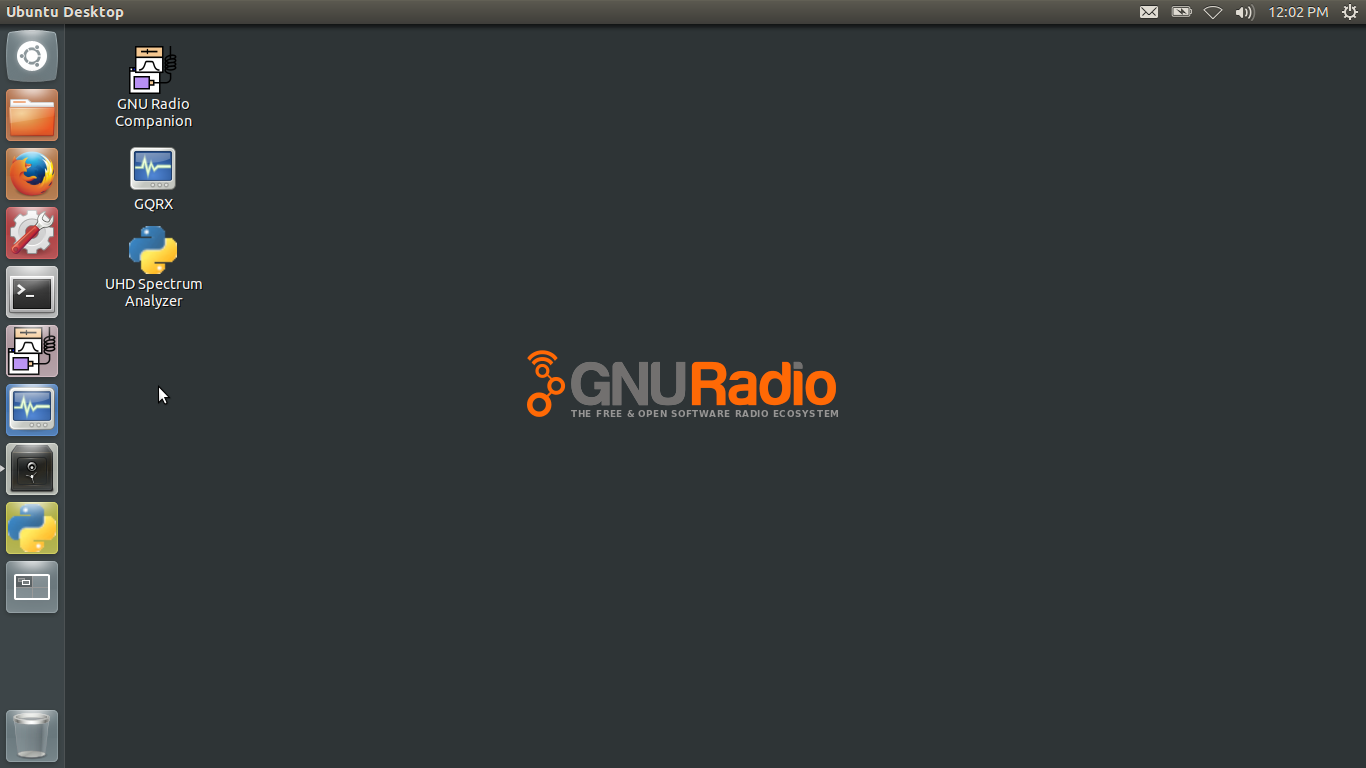
\includegraphics[height=5em]{grlivedvd}
    \hspace{1em}
    \includegraphics<3->[height=5em]{pybombs_logo}
    \hspace{1em}
    \includegraphics<4->[height=5em]{srcbuild}
\end{frame}
% Note: Show synaptic

\begin{frame}
  \frametitle{PyBOMBS --- The apt-get of GNU Radio}
  \begin{itemize}
    \item Installs GNU Radio, Hardware Drivers and OOTs for you!
    \item Sets up environment variables etc.\ for you!
    \item Currently available at: \texttt{http://gnuradio.org/pybombs}
    \item Modules are added by PyBOMBS maintainers in form of lightweight recipes
    \item Rewrite happening, PyBOMBS 2.0 to be released this year
  \end{itemize}
\end{frame}

\begin{frame}
  \frametitle{PyBOMBS 2.0}

  \begin{columns}[c]
    \column[T]{9cm}

  \begin{itemize}
    \item Still Alpha
    \item Features:
      \begin{itemize}
        \item Installable
        \item Multiple prefixes, each with its own configuration
        \item Multiple recipe remotes, per system, per user or per prefix
        \item Easy cross-compiling
      \end{itemize}
    \item Action happening at: \texttt{github.com/gnuradio/pybombs2}
  \end{itemize}

    \column[T]{2cm}

  
\includegraphics[width=\textwidth]{pybombs_logo}

  \end{columns}
\end{frame}
% NOTE: Don't Demo PyBOMBS :(

\begin{frame}
  \frametitle{Source Builds}
  \begin{itemize}
    \item Useful for development on GNU Radio itself
    \item Requirements:
      \begin{enumerate}
        \item Install all dependencies (Boost, UHD, QT, \ldots)
        \item Run \texttt{cmake \&\& make \&\& make install}
        \item Et Voilà! You're done! (or not)
      \end{enumerate}
  \end{itemize}
\end{frame}

\section{Resources}

\begin{frame}
  \frametitle{GNU Radio Companion}
  \begin{itemize}
    \item Graphical front-end for GNU Radio (its face)
    \item Powerful graphical widgets for live inspection of signals/data
    \item Ignore GRC at your own peril
  \end{itemize}
  \begin{center}
  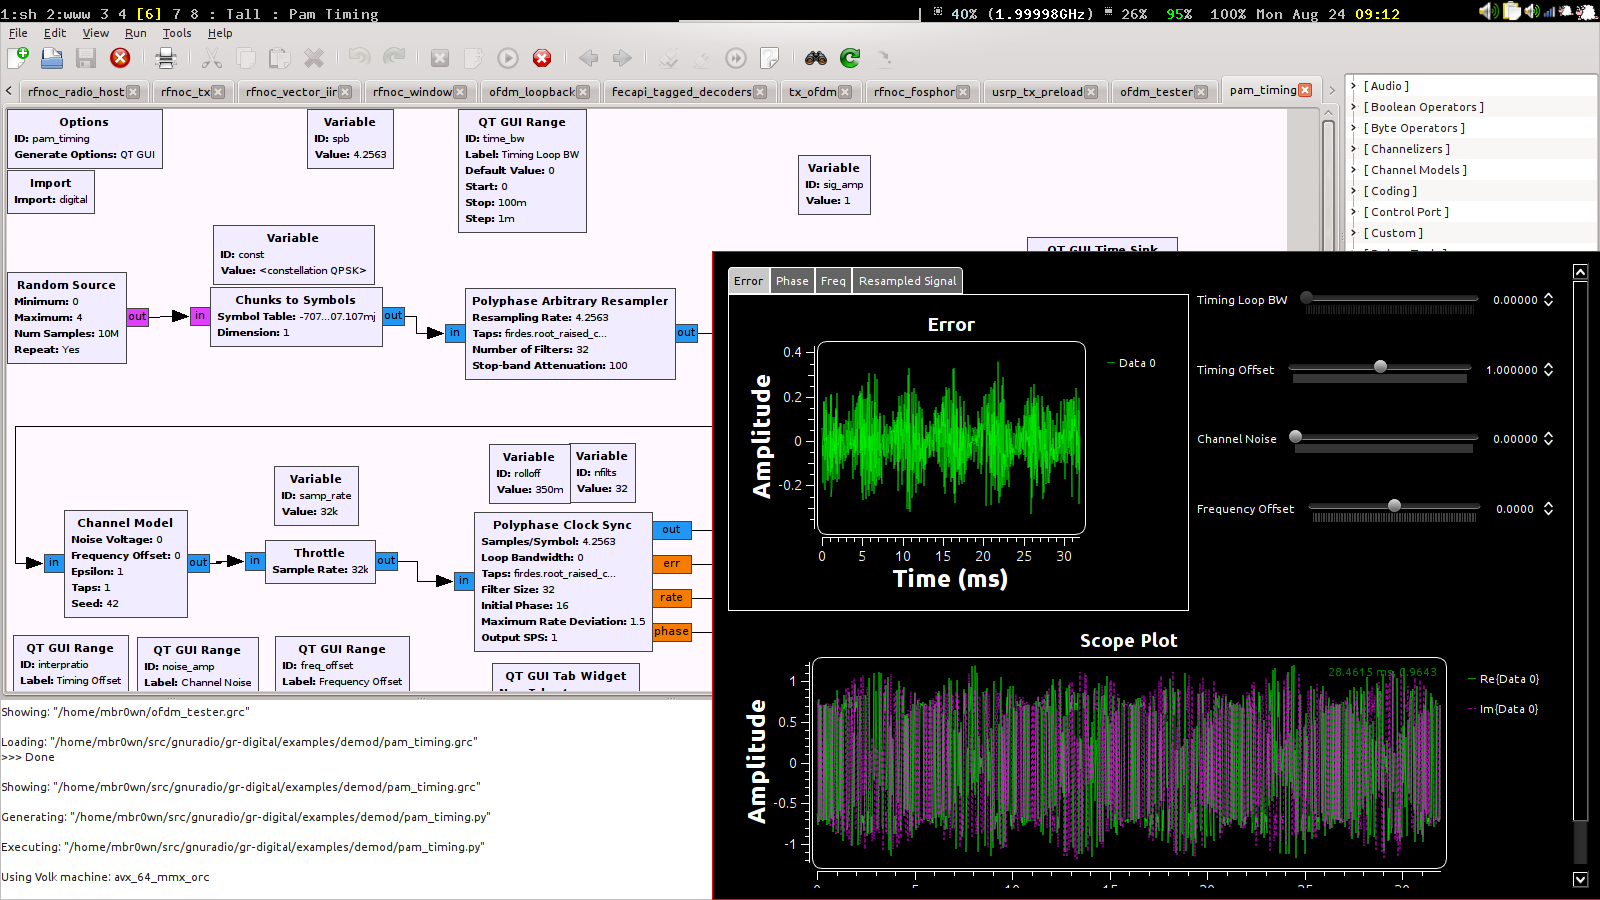
\includegraphics[height=4cm]{grc}
  \end{center}
\end{frame}

\begin{frame}
  \frametitle{CGRAN}

  \begin{columns}[c]
    \column[T]{9cm}

  \begin{itemize}
    \item Spiritual Cousin of CTAN, CPAN\ldots
    \item Recently rewritten by the CGRAN Special Forces (main contributors: Nathan + Ravi)
    \item Easy access to the entire free \& open software radio ecosystem
    \item Automatically generated website listing most OOT modules
    \item Between CGRAN and PyBOMBS, finding and installing modules should be a simple task
  \end{itemize}

    \column[T]{2cm}

  
\includegraphics[width=\textwidth]{cgran_logo}

  \end{columns}

\end{frame}
% Note: Show cgran.org

\begin{frame}
  \frametitle{First Steps: Guided Tutorials}
  \begin{itemize}
    \item Gentle introduction to GNU Radio (and even some DSP)
    \item Find these online on our wiki
    \item Comes with a free set of codes: \texttt{gr-tutorial}
  \end{itemize}
\end{frame}
% Note: show GTs

\begin{frame}
  \frametitle{Where do I learn about these blocks?}
  \begin{itemize}
    \item Read our fine manual!
      \begin{itemize}
        \item \texttt{http://gnuradio.org/doc/}
      \end{itemize}
    \item All blocks are browsable through several paths, and searchable
    \item GRC provides docs, too
  \end{itemize}
\end{frame}

\section{Starting to Code}
\begin{frame}[fragile]
  \frametitle{\texttt{gr\_modtool} --- The Swiss Army Knife of modules}
  \begin{itemize}
    \item Modify and create your OOTs from the command line
      \begin{itemize}
        \item Unfortunately, only the command line at this time
      \end{itemize}
    \item Create, remove, disable, enable blocks
    \item Never write any boilerplate code again!
  \end{itemize}
\end{frame}

\begin{frame}
  \frametitle{Writing blocks: A core skill of developing SDR}
  \begin{itemize}
    \item \texttt{gr\_modtool} tries to make this as easy as possible
    \item Languages available:
      \begin{itemize}
        \item Python, for fast \& easy dev
        \item C++, for highest performance
      \end{itemize}
  \end{itemize}
\end{frame}
% Note: Coding exercise here
% - gr_modtool help
% - Build square block in C++
% - Build whatever in Python (fizzbuzz, remember the zero)

\begin{frame}
  \frametitle{Where do I learn how to use all these blocks?}
  \begin{itemize}
    \item Where do I learn how to do all this wireless communications stuff?
    \item Which codez do I put into my \\ \texttt{<+ do signal processing here +>}?
    \item<2-> Well\ldots
    \item<3-> Ask Jeff (next talk)
  \end{itemize}
  \begin{center}
    \includegraphics<2->[height=4cm]{books.jpg}
  \end{center}
\end{frame}

\begin{frame}
  \frametitle{Getting Help --- Interacting with other People}
  \begin{itemize}
    \item discuss-gnuradio, usrp-users mailing lists
    \item Very responsive!
    \item IRC\@: \#gnuradio on Freenode
    \item Join the discussions!
    \item But first, read the wiki page on reporting errors, etc.!
  \end{itemize}
\end{frame}
% NOTE: Open mailing/reporting errors pages

\section{Becoming a Developer}
\begin{frame}
  \frametitle{Improving GNU Radio}
  \begin{itemize}
    \item You've found a bug? Something's bothering you?
    \item Fix it!
      \begin{itemize}
        \item Actual bugs
        \item Missing features
        \item Bad docs
        \item Unintuitive coding
      \end{itemize}
  \end{itemize}
\end{frame}
% NOTE: Contribution guide

\section{The Community}
\begin{frame}
  \frametitle{The Community}
  \begin{itemize}
    \item Am I supposed to do this all alone?
    \item (Also, I'm running out of shirts)
    \item<2-> No!
    \item<2-> See \texttt{gnuradio.spreadshirt.\{com, de\}}
    \item<3-> There's a big community, join it!
    \item<3-> There's the conference, and also local meetings, hackfests\ldots
  \end{itemize}
\end{frame}
% NOTE: Open webshop

\begin{frame}
  \frametitle{Conclusion}
  \begin{itemize}
    \item SDR is a very hard topic
    \item But GNU Radio is there to make it easier
    \item Getting started with GNU Radio, writing first blocks etc.\ is well documented at this point
      \begin{itemize}
        \item (and if it's not, maybe you can help us improve it!)
      \end{itemize}
    \item And after that, we have a great community
  \end{itemize}
\end{frame}

\end{document}
